\documentclass{standalone}

\usepackage{tikz}
\usetikzlibrary{arrows.meta,angles,quotes,decorations.pathreplacing,positioning}

\usepackage{newtx}
\usepackage{bm}
\renewcommand\mathbf\bm

\begin{document}
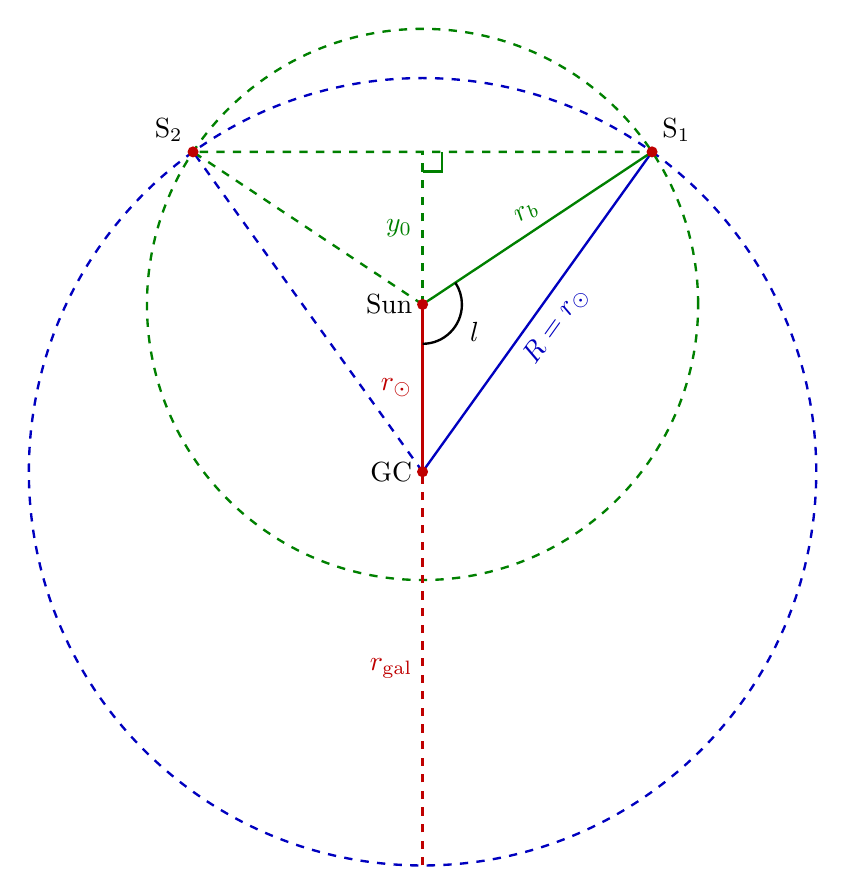
\begin{tikzpicture}[line width=0.3mm]
    \coordinate [label=left:GC] (O) at (0,0);
    \coordinate [label=left:Sun] (S) at (0,2.125);
    \draw [blue!75!black,dashed] (O) circle [radius=5cm];
    \draw [green!50!black,dashed] (S) circle [radius=3.5cm];
    \coordinate [label=above right:$\mathrm{S}_1$] (S1) at (2.91480595,4.0625);
    \coordinate [label=above left:$\mathrm{S}_2$] (S2) at (-2.91480595,4.0625);
    \coordinate (H) at (0,4.0625);
    \draw [red!75!black] (O) -- (S) node [midway,left] {$r_\odot$};
    \draw [red!75!black,dashed] (0,-5) -- (O) node [midway,left] {$r_{\mathrm{gal}}$};
    \draw [blue!75!black] (O) -- (S1) node [midway,below,sloped] {$R=r_\odot$};
    \draw [green!50!black] (S) -- (S1) node [midway,above,sloped] {$r_b$};
    \draw [blue!75!black,dashed] (O) -- (S2);
    \draw [green!50!black,dashed] (S) -- (S2) -- (S1);
    \draw [green!50!black,dashed] (S) -- (H) node [midway,left] {$y_0$};
    \path (O) -- (S) -- (S1) pic ["$l$",draw,angle radius=0.5cm,angle eccentricity=1.5] {angle = O--S--S1};
    \path (S) -- (H) -- (S1) pic [draw,angle radius=0.25cm,green!50!black,] {right angle = S--H--S1};
    \fill [color=red!75!black] (O) circle (2pt);
    \fill [color=red!75!black] (S) circle (2pt);
    \fill [color=red!75!black] (S1) circle (2pt);
    \fill [color=red!75!black] (S2) circle (2pt);
\end{tikzpicture}
\end{document}